Nykyisen järjestelmän suurin ongelma on sen laajennettavuuden vaikeus. Jos Sikteerin lisäksi halutaan kehittää muita käyttäjien tunnistusta vaativia web-sovelluksia, joudutaan niihin tekemään käyttäjän tunnistaminen Sikteerin tavoin. Eräs suunnitteilla oleva palvelu on käyttäjien palvelunhallinta, jota kautta jäsenet voisivat lisätä itselleen jäsenmaksuun kuuluvia palveluita, kuten sähköpostialiaksia ja domaineja. Jäsenet kirjautuvat palveluhallintaan henkilökohtaisella Kapsi ry:n käyttäjätunnuksella.

Kun nykyiseen arkkitehtuuriin liitetään uusi web-sovellus, joudutaan luomaan uusi tietokanta, johon on kopioitu käyttäjien tunnukset ja salasanat. Jotta uusien web-sovellusten liittäminen on mahdollista, täytyy niillä olla tapa tunnistaa käyttäjä. Keskitetyn tunnistautumispalvelun avulla uudet sovellukset voivat tunnistaa käyttäjän ilman, että salasanoja täytyy kopioida uuteen tietokantaan.

Tietojen synkronointi on ongelma nykyisessä arkkitehtuurissa, vaikka siihen ei lisättäisi yhtään uutta palvelua. Varsinainen käyttäjähallinta on Sikteerin ulkopuolisessa LDAP-tie\-to\-kan\-nas\-sa, josta data synkronoidaan Sikteerin omaan tietokantaan. Käyttäjän tietoihin tallennettujen tunnistetietojen perusteella Sikteeri tunnistaa käyttäjät. Tulevaisuudessa tietojen synkronointia ei haluta tehdä, vaan käyttäjien tunnistetiedot halutaan säilyttää vain LDAP-tietokannassa. Koska käyttäjätietokantaan on tallennettu henkilökohtaista dataa, kuten henkilötunnuksia, halutaan integroinnit siihen pitää mahdollisimman vähälukuisina.

Kuvassa \ref{kapsi_nykyinen_uusi} on nykyisten hallintatyökalujen arkkitehtuuri, kun siihen on lisätty keskitetty tunnistautumispalvelu. Tunnistautumispalvelu on ainoa komponentti, jolla on pääsy LDAP-tietokantaan. Sikteerin tietokannassa säilytetään vain listaa käyttäjätunnuksista, joilla on oikeus käyttää järjestelmää. Kaikki muut käyttäjään liittyvät tiedot ovat vain LDAP-tietokannassa ja ne haetaan sieltä tarvittaessa tunnistautumispalvelun avulla.

\begin{figure}[ht]
\centering
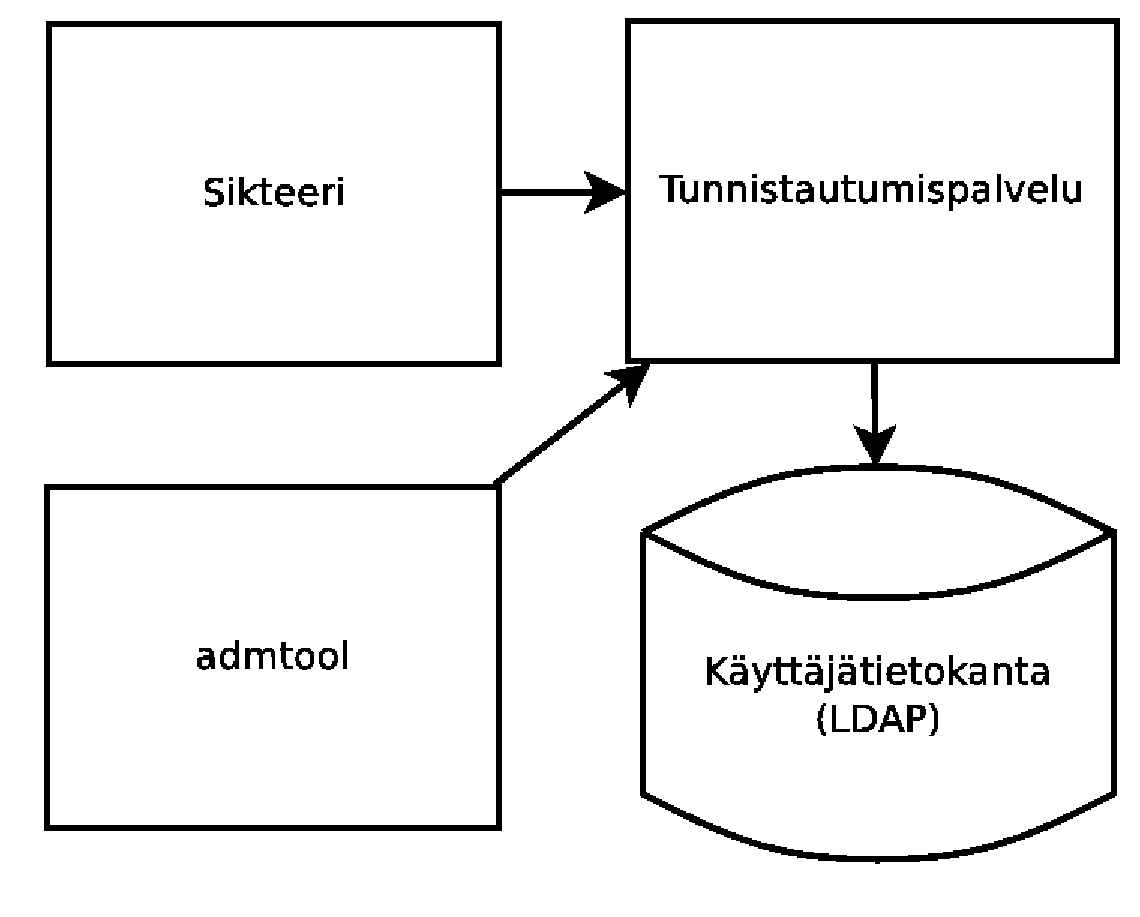
\includegraphics[width=.7\textwidth]{toteutus/muutostarve/kapsi_uusi.eps}
\caption{Keskitettyä tunnistautumispalvelua käyttävä hallintatyökalujen arkkitehtuuri.}%
\label{kapsi_nykyinen_uusi}
\end{figure}

Sikteeri on vuosien varrella paisunut yleiseksi toiminnanohjausjärjestelmäksi, jonka arkkitehtuuria kehittäjät haluaisivat viedä palvelusuuntautuneiden arkkitehtuurien suuntaan. Tällöin esimerkiksi laskutukseen tai jäsenrekisteriin liittyvät tehtävät voitaisiin toteuttaa omana palveluna. Kuvassa \ref{kapsi_uusi} on esitetty tavoiteltu arkkitehtuuri, jossa Sikteerin laskutus- ja jäsenrekisteripalvelut ovat itsenäisiä web-sovelluksia ja joiden rinnalla on admtool-komentorivityökalu sekä käyttäjien palvelunhallinta. Seuraavassa luvussa esiteltävän arkkitehtuurin puitteissa ei oteta kantaa Sikteerin palveluperustaiseen arkkitehtuuriin, vaan pyritään löytämään ratkaisu, joka mahdollistaa myös ko. arkkitehtuurimuutoksen tulevaisuudessa.

\begin{figure}[ht]
\centering
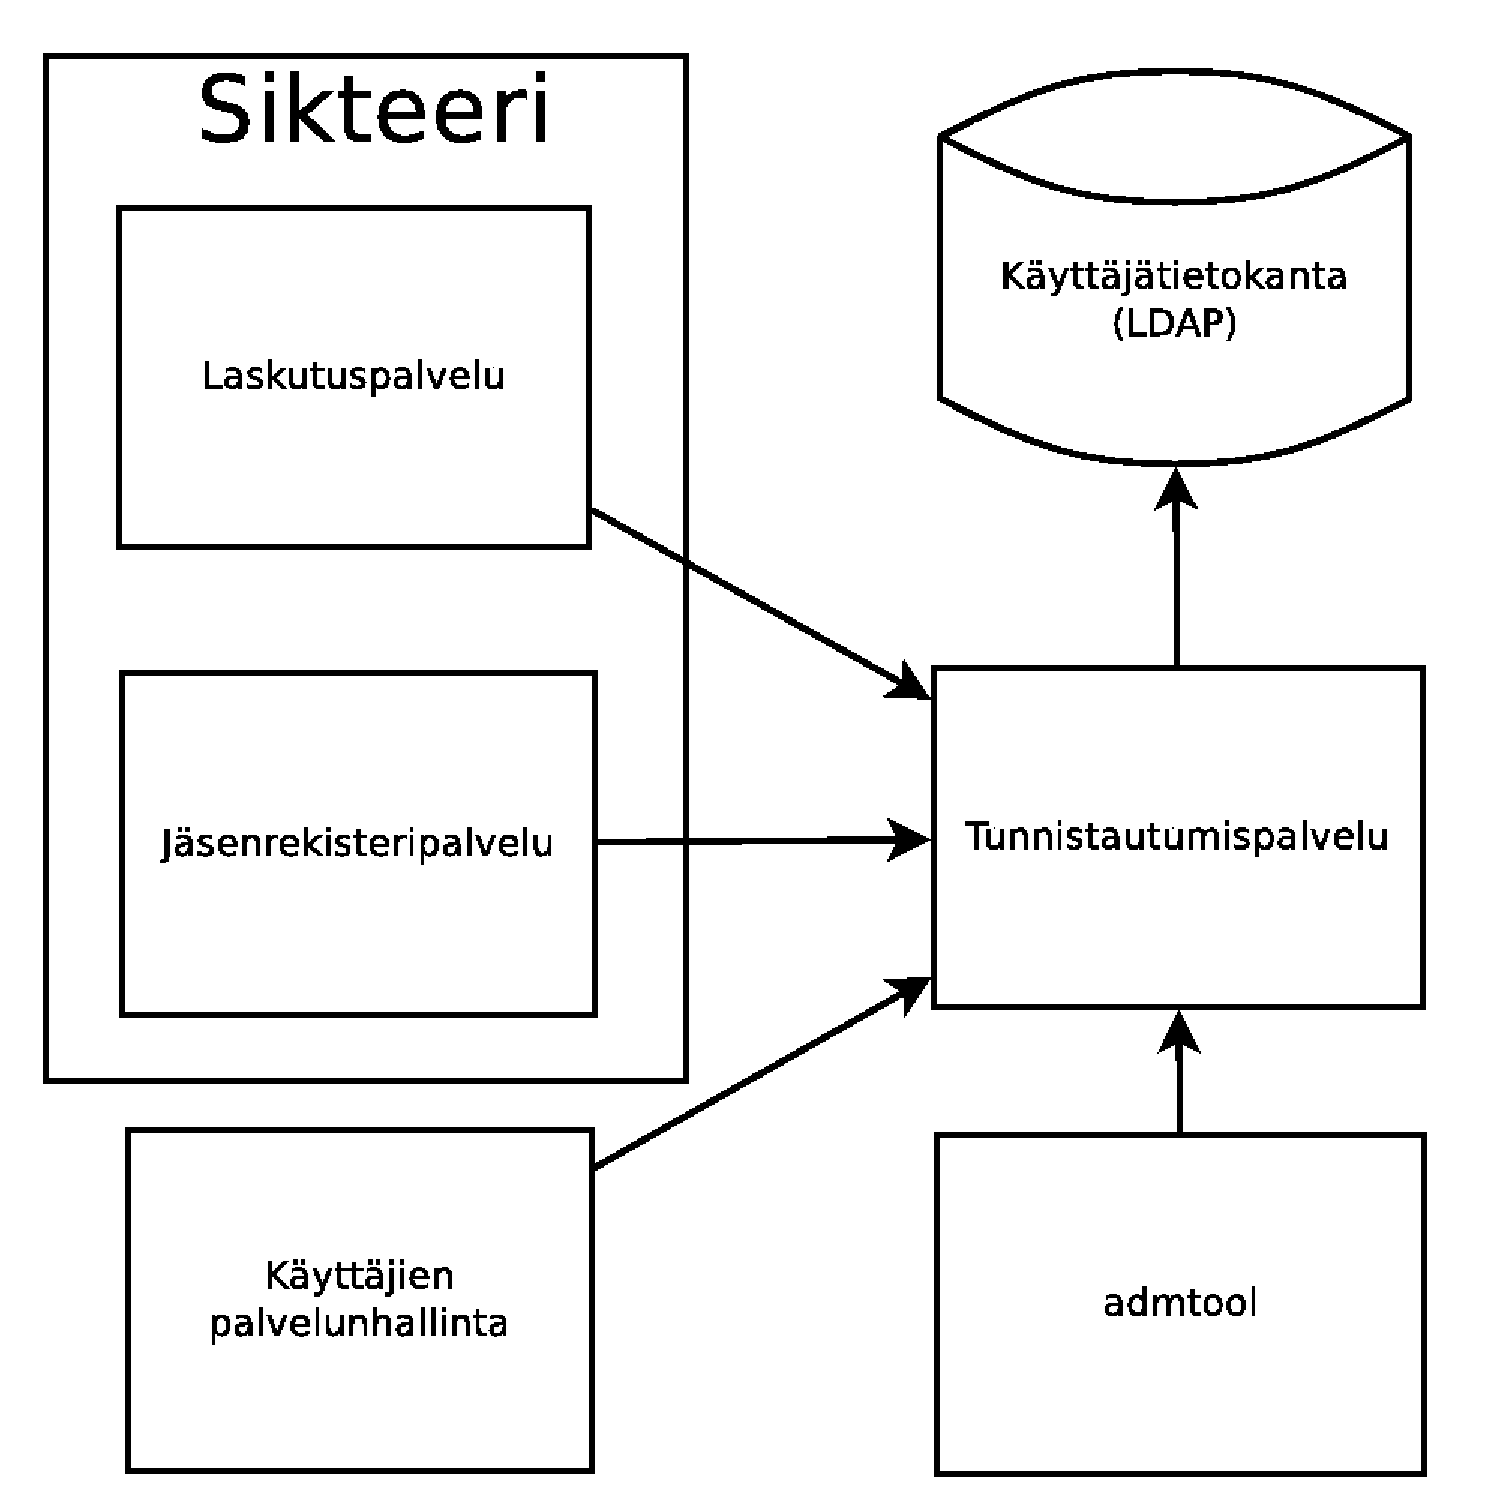
\includegraphics[width=.7\textwidth]{toteutus/muutostarve/kapsi_uusi_soa.eps}
\caption{Palveluperustaisten arkkitehtuurien mukainen kuvaus Kapsin järjestelmästä.}%
\label{kapsi_uusi}
\end{figure}